%% PNAStmpl.tex
%% Template file to use for PNAS articles prepared in LaTeX
%% Version: Apr 14, 2008


%%%%%%%%%%%%%%%%%%%%%%%%%%%%%%
%% BASIC CLASS FILE
%% PNAStwo for two column articles is called by default.
%% Uncomment PNASone for single column articles. One column class
%% and style files are available upon request from pnas@nas.edu.
%% (uncomment means get rid of the '%' in front of the command)

%\documentclass{pnasone}
\documentclass{pnastwo}

%%%%%%%%%%%%%%%%%%%%%%%%%%%%%%
%% Changing position of text on physical page:
%% Since not all printers position
%% the printed page in the same place on the physical page,
%% you can change the position yourself here, if you need to:

% \advance\voffset -.5in % Minus dimension will raise the printed page on the
                         %  physical page; positive dimension will lower it.

%% You may set the dimension to the size that you need.

%%%%%%%%%%%%%%%%%%%%%%%%%%%%%%
%% OPTIONAL GRAPHICS STYLE FILE

%% Requires graphics style file (graphicx.sty), used for inserting
%% .eps files into LaTeX articles.
%% Note that inclusion of .eps files is for your reference only;
%% when submitting to PNAS please submit figures separately.

%% Type into the square brackets the name of the driver program
%% that you are using. If you don't know, try dvips, which is the
%% most common PC driver, or textures for the Mac. These are the options:

% [dvips], [xdvi], [dvipdf], [dvipdfm], [dvipdfmx], [pdftex], [dvipsone],
% [dviwindo], [emtex], [dviwin], [pctexps], [pctexwin], [pctexhp], [pctex32],
% [truetex], [tcidvi], [vtex], [oztex], [textures], [xetex]

%\usepackage[dvips]{graphicx}

%%%%%%%%%%%%%%%%%%%%%%%%%%%%%%
%% OPTIONAL POSTSCRIPT FONT FILES

%% PostScript font files: You may need to edit the PNASoneF.sty
%% or PNAStwoF.sty file to make the font names match those on your system.
%% Alternatively, you can leave the font style file commands commented out
%% and typeset your article using the default Computer Modern
%% fonts (recommended). If accepted, your article will be typeset
%% at PNAS using PostScript fonts.

% Choose PNASoneF for one column; PNAStwoF for two column:
%\usepackage{PNASoneF}
\usepackage{PNAStwoF}

%%%%%%%%%%%%%%%%%%%%%%%%%%%%%%
%% ADDITIONAL OPTIONAL STYLE FILES

%% The AMS math files are commonly used to gain access to useful features
%% like extended math fonts and math commands.

\usepackage{amssymb,amsfonts,amsmath}

%\usepackage{subcaption}
\graphicspath{ {paper_figures2/} }

%\usepackage{sansmath}

%\usepackage[font={sf, small}]{caption}

%%%%%%%%%%%%%%%%%%%%%%%%%%%%%%
%% OPTIONAL MACRO FILES
%% Insert self-defined macros here.
%% \newcommand definitions are recommended; \def definitions are supported

%\newcommand{\mfrac}[2]{\frac{\displaystyle #1}{\displaystyle #2}}
%\def\s{\sigma}

\DeclareMathSizes{9}{8}{7}{7}

\DeclareMathOperator*{\argmin}{arg\,min}

\makeatletter
\newcommand{\customlabel}[2]{%
\protected@write \@auxout {}{\string \newlabel {#1}{{#2}{}}}}
\makeatother

%%%%%%%%%%%%%%%%%%%%%%%%%%%%%%
%% Don't type in anything in the following section:
%%%%%%%%%%%%
%% For PNAS Only:
\contributor{Submitted to Proceedings
of the National Academy of Sciences of the United States of America}
\url{www.pnas.org/cgi/doi/10.1073/pnas.0709640104}
\copyrightyear{2008}
\issuedate{Issue Date}
\volume{Volume}
\issuenumber{Issue Number}
%%%%%%%%%%%%

\begin{document}

%%%%%%%%%%%%%%%%%%%%%%%%%%%%%%


%% For titles, only capitalize the first letter
%% \title{Almost sharp fronts for the surface quasi-geostrophic equation}

\title{Reduction of biological imaging data}


%% Enter authors via the \author command.
%% Use \affil to define affiliations.
%% (Leave no spaces between author name and \affil command)

%% Note that the \thanks{} command has been disabled in favor of
%% a generic, reserved space for PNAS publication footnotes.

%% \author{<author name>
%% \affil{<number>}{<Institution>}} One number for each institution.
%% The same number should be used for authors that
%% are affiliated with the same institution, after the first time
%% only the number is needed, ie, \affil{number}{text}, \affil{number}{}
%% Then, before last author ...
%% \and
%% \author{<author name>
%% \affil{<number>}{}}

%% For example, assuming Garcia and Sonnery are both affiliated with
%% Universidad de Murcia:
%% \author{Roberta Graff\affil{1}{University of Cambridge, Cambridge,
%% United Kingdom},
%% Javier de Ruiz Garcia\affil{2}{Universidad de Murcia, Bioquimica y Biologia
%% Molecular, Murcia, Spain}, \and Franklin Sonnery\affil{2}{}}

\author{Carmeline~J.~Dsilva\affil{1}{Department of Chemical and Biological Engineering, Princeton University, Princeton, New Jersey, USA},
Bomyi~Lim\affil{1}{},
Thomas~J.~Levario\affil{2}{School of Chemical and Biomolecular Engineering, Georgia Institute of Technology, Atlanta, Georgia, USA},
Hang~Lu\affil{2}{},
Amit~Singer\affil{3}{Department of Mathematics, Princeton University, Princeton, New Jersey, USA} \affil{4}{Program in Applied and Computational Mathematics, Princeton University, Princeton, New Jersey, USA},
Stanislav~Y.~Shvartsman\affil{1}{} \affil{5}{Lewis-Sigler Institute for Integrative Genomics, Princeton University, Princeton, New Jersey, USA},
\and
Ioannis~G.~Kevrekidis\affil{1}{} \affil{4}{Program in Applied and Computational Mathematics, Princeton University, Princeton, New Jersey, USA}}

\contributor{Submitted to Proceedings of the National Academy of Sciences
of the United States of America}

%% The \maketitle command is necessary to build the title page.
\maketitle

%%%%%%%%%%%%%%%%%%%%%%%%%%%%%%%%%%%%%%%%%%%%%%%%%%%%%%%%%%%%%%%%
\begin{article}

\begin{abstract}

We demonstrate how data reduction techniques can effectively organize large sets of biological images. 
%
We use existing algorithms to both register images within a data set so that they are in a consistent frame of reference, as well as extract meaningful structure within the image data set.
%
We illustrate the utility of such algorithms using two data sets from a study of {\it Drosophila} emrbyogenesis.
%
Here, we show that we can temporally order the images to obtain a representative picture of the embryogenesis dynamics. 	
%
In general, these algorithms allow us to extract meaningful structure from imaging data sets where the patterns are not known {\it a priori}. 


\end{abstract}


%% When adding keywords, separate each term with a straight line: |
\keywords{temporal ordering | image registration}

%% Optional for entering abbreviations, separate the abbreviation from
%% its definition with a comma, separate each pair with a semicolon:
%% for example:
%% \abbreviations{SAM, self-assembled monolayer; OTS,
%% octadecyltrichlorosilane}

% \abbreviations{}

%% The first letter of the article should be drop cap: \dropcap{}
%\dropcap{I}n this article we study the evolution of ''almost-sharp'' fronts

%% Enter the text of your article beginning here and ending before
%% \begin{acknowledgements}
%% Section head commands for your reference:
%% \section{}
%% \subsection{}
%% \subsubsection{}


Imaging data is becoming increasingly prevalent in biology research.
%
General motivation about biology data ...

Need methods to organize data, visualize, ...

REDUCTION is important, reduction because of symmetry and reduction because of content

There are a bunch of recent techniques- some established (like dmaps), some very fresh, like synchronization or VDMaps,  that have had their own reasons to be developed but they are as if tailor made for what we would want to do



\section{Results and Discussion}

We apply the methods to two imaging data sets from a study of {\it Drosophila} embryogenesis.
%
The first data set (Figure~\ref{subfig:raw_data1}) is from stage 5, when cellularization occurs. 
%
The second data set (Figure~\ref{subfig:raw_data2}) is from the end of stage 5 to stage 7, which captures formation of the ventral furrow and gastrulation.
%
In both of these data sets, each image is taken from a different embryo, fixed at a different developmental time and imaged in a different rotational orientation.
%
We would like to organize these data sets in a meaningful and informative way.
%
This requires rotating and translating each image so the set is in a consistent frame of reference ({\it registration}), and then organizing the images. 
%
For these data sets, we know (by experimental design) that the main source of variability comes from the different developmental time of each image.
%
We will show that the algorithms can effectively order the images in time and therefore give us meaningful picture of the underlying developmental dynamics. 


\subsection{Image Registration}

Because each embryo is imaged in a different orientation, the first task is to align or {\em register} the images so that they are in a consistent frame of reference.
%
We use angular synchronization \cite{singer2011angular} to register our images with respect to translations and rotations. 
%
The task of image registration has been broadly studied in a variety of contexts (see, for example, ...).
%
We chose to use angular synchronization because it is a very general technique which requires no {\em a priori} knowledge of a good template image or feature points. 
%
Therefore, this algorithm can readily be extended to other imaging data sets. 
%
Implementation details are given in the {\it SI appendix}. 

The images in Figure \ref{subfig:ordered_data1} have been registered using angular synchronization.
%
The important features that our eye can visually detect (e.g., the green Dorsal peaks) have been aligned, even though the algorithm does not require explicit identification of such features.

\begin{figure}[t]
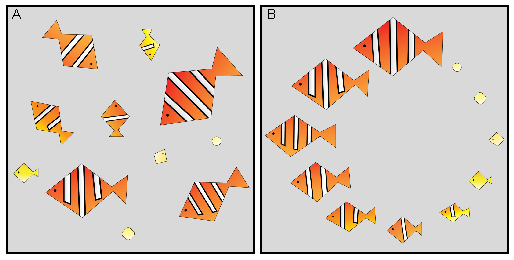
\includegraphics[width=8.4cm]{fig1}
\caption{{\it (A)} Fish, each in a different orientation and a different stage of development. {\it (B)} Fish, now rotationally registered and temporally ordered. For this caricature, the registration and ordering is easy to do ``by hand" because the data set is small and the developmental changes are easy to recognize.}
%\label{fig:fish}
\customlabel{fig:fish}{1}
\customlabel{subfig:fish_unordered}{\ref{fig:fish}{\it A}}
\customlabel{subfig:fish_ordered}{\ref{fig:fish}{\it B}}
\end{figure}

\begin{figure}[t]
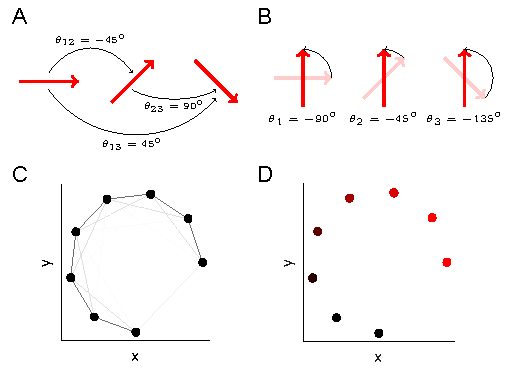
\includegraphics[width=8.4cm]{fig2} 
\caption{{\it (A)} Fluorescent images of {\it Drosophila} embryos in stage 5. Each embryo has been stained for Dorsal (green) and dpERK (red). Each image is of a different embryo in a different rotational orientation.  {\it (B)} Selected image from data set. {\it (C)} Profile of Dorsal (green) and dpERK (red) around the circumference of the embryo in {\it B}. }
\customlabel{fig:data1}{2}
\customlabel{subfig:raw_data1}{\ref{fig:data1}{\it A}}
\customlabel{subfig:select_image}{\ref{fig:data1}{\it B}}
\customlabel{subfig:1d_profile}{\ref{fig:data1}{\it C}}
\end{figure}

\subsection{Temporal Ordering using Principal Component Analysis}



After registering our images so that they are in a consistent frame of reference, we would like to organize our images to extract meaningful patterns and structure. 
%
Although our images are inherently high-dimensional (number of pixels $\times$ number of channels), we assume that there are only a few modes/directions of variability.
%
We will use dimensionality reduction techniques to extract these main directions of variability and efficiently organize our images.
%
%In our examples, we assume that the main source of variability in this data is due to time/developmental dynamics. 
%
%We will show that dimensionality reduction techniques uncover a one-dimensional parameterization/organization of our images, and that the images are temporally ordered in this parameterization.

Principal component analysis (PCA) \cite{shlens2005tutorial} is arguably the most common dimensionality reduction technique.
%
PCA extracts the main directions/modes of variability in a data set. 
%
We applied PCA to the data set shown in Figure~\ref{subfig:raw_data1}.
%
The first two modes, or eigenimages, are shown in Figure~\ref{subfig:eigenimage1}~and~\ref{subfig:eigenimage2}.
%
Clearly, these modes extract/capture meaningful features that we can visually detect in the data set. 
%
We can plot the data projected onto the first two eigenimages; this is shown in Figure~\ref{subfig:PCA_12}.
%
From this plot, we can see that the data fall effectively on a one-dimensional curve that is parameterized by the first projection coefficient.
%
Therefore, an approrpiate way to organize the images would be to order them according to the first projection coefficient. 

Figure~\ref{subfig:ordered_data1} shows the images from Figure~\ref{subfig:raw_data1}, now ordered by the first projection coefficient.
%
We can now easily see the relevant structure in the data set:
the red peaks grow in intensity.
%
Furthermore, for this data set, we know what the relevant structure is.
%
The data consists of embryos fixed at different developmental times. 
%
During stage 5, we can measure the developmental time based on the monotonic progress of cellularization (Figure~\ref{subfig:membranes}) \cite{figard2013plasma}.%; this helps validate our vector diffusion map-based ordering.
%
The ordering we extract using the first eigenimage is consistent with the temporal ordering of the images using cellularzation.
%
Quantitatively, the rank correlation coefficient between these two orderings is 0.9199.
%
The two methods for registration and ordering can be visually compared through the sequences of one-dimensional profiles extracted from the circumference of the embryos, shown in Figures~\ref{subfig:1d_membranes}~and~\ref{subfig:1d_vdm}.
%
The general trends are consistent:
both green  and red peaks are aligned, and the red peaks grow as a function of time/first PCA projection coefficient.

Although PCA can successfully order the data set shown in Figure \ref{subfig:raw_data1}, in general, such data is not guaranteed to lie in a low-dimensional, {\it linear} subspace.
%
When the data have nonlinear structure, PCA may not provide the most parsimonious organization of the data.
%
This can be seen in the late images of Figure~\ref{subfig:ordered_data1};
images where the ventral furrow begins to form are interspersed with images containing no obvious dent.
%
This is because the dynamics at later stages are nonlinear and and not effectively described by a single eigenimage.
%
We can see this from the projection onto the first two eigenimages, shown in Figure~\ref{subfig:PCA_12}.
%
The data clearly lie on a one-dimensional, {\em nonlinear} curve.
%
This motivates us to use nonlinear dimensionality reduction techniques to organize our data.


\begin{figure}[t]
\raisebox{3.5cm}{{\figtextfont A}}
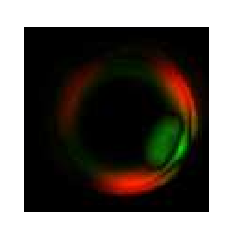
\includegraphics[width=4.2cm]{PCA_eigenimage1}
\raisebox{3.5cm}{{\figtextfont B}}
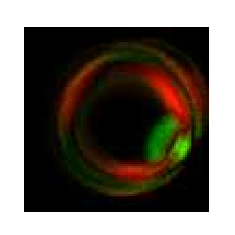
\includegraphics[width=4.2cm]{PCA_eigenimage2}

\raisebox{4cm}{{\figtextfont C}}
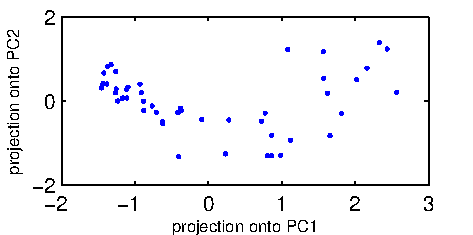
\includegraphics[width=8.4cm]{PCA_12}

\raisebox{8cm}{{\figtextfont D}}
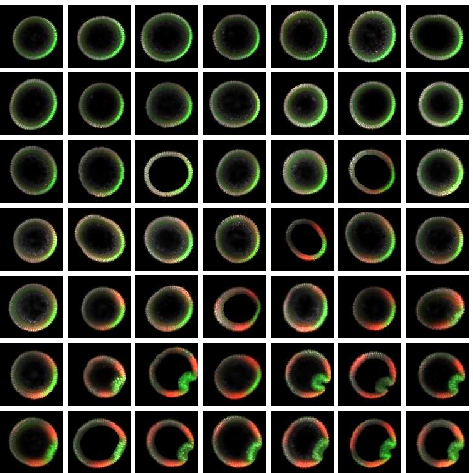
\includegraphics[width=8.4cm]{PCA_ordered}
\caption{{\it (A)} First eigenimage from the data set shown in Figure~\ref{subfig:raw_data1}. {\it (B)} Second eigenimage from the data set shown in Figure~\ref{subfig:raw_data1}. {\it (B)} Projection of  data set shown in Figure~\ref{subfig:raw_data1} onto the first two eigenimages. {\it (D)} Ordering of  data set shown in Figure~\ref{subfig:raw_data1} by the first projection coefficient. }
\customlabel{fig:data1b}{3}
\customlabel{subfig:eigenimage1}{\ref{fig:data1b}{\it A}}
\customlabel{subfig:eigenimage2}{\ref{fig:data1b}{\it B}}
\customlabel{subfig:PCA_12}{\ref{fig:data1b}{\it C}}
\customlabel{subfig:ordered_data1}{\ref{fig:data1b}{\it D}}
\end{figure}

\begin{figure}[t]
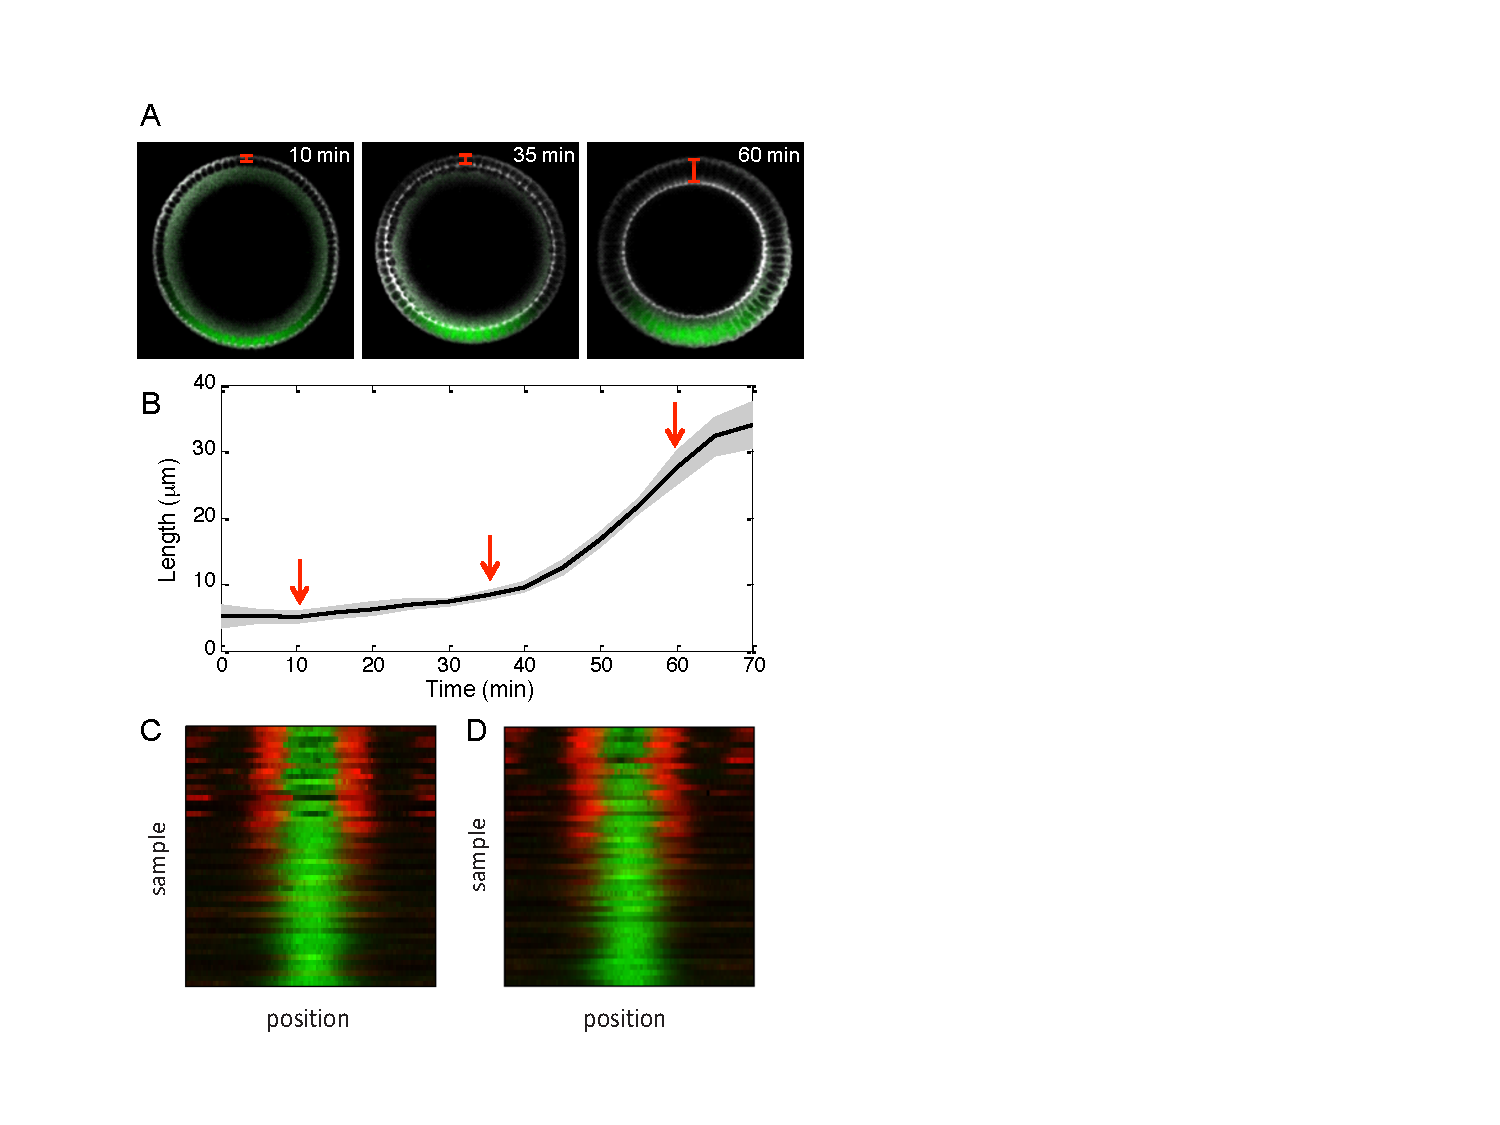
\includegraphics[width=8.4cm]{fig6}
\caption{{\it (A)} Images, stained for membranes (gray) and Dorsal (green) at different levels of development. {\it (B)} Membrane length as a function of time. The points corresponding to the images in {\it A} are indicated with arrows. {\it (C)} The one-dimensional concentration profiles, registered by peak Dorsal fluorescence and ordered by membrane length. {\it (D)} The one-dimensional concentration profiles corresponding to the automatically registered and ordered images in Figure~\ref{fig:images_ordered}. }
%\label{fig:membrane_compare}
\customlabel{fig:membrane_compare}{4}
\customlabel{subfig:membranes}{\ref{fig:membrane_compare}{\it A}}
\customlabel{subfig:membrane_curve}{\ref{fig:membrane_compare}{\it B}}
\customlabel{subfig:1d_membranes}{\ref{fig:membrane_compare}{\it C}}
\customlabel{subfig:1d_vdm}{\ref{fig:membrane_compare}{\it D}}
\end{figure}

\subsection{Temporal Ordering Using Diffusion Maps}

We can use diffusion maps \cite{coifman2005geometric} to analyze data sets with nonlinear structure.
%
Diffusion maps is similar to PCA, in that it aims uncover low-dimensional structure in high-dimensional data.
%
However, unlike PCA, diffusion maps is a {\it nonlinear} reduction technique. 

Figure~\ref{subfig:raw_data2} shows a data set of images from stages 5--7.
%
Clearly, the dynamics are significantly more complex than the dynamics in Figure~\ref{subfig:raw_data1}, and the first eigenimage will not capture all of the relevant dynamics.
%
However, we can still use diffusion maps to temporally order the data.
%
In addition, we can combine the steps image registration and temporal ordering using vector diffusion maps. 

Figure~\ref{subfig:ordered_data2} shows the images in Figure~\ref{subfig:raw_data2}, now registered and ordered using vector diffusion maps \cite{singer2012vector}.
%
Unlike the images in Figure~\ref{subfig:raw_data1}, 
for Figure~\ref{fig:data2}, we have no time marker with which to validate our orderings.
%
However, there are noticeable features in the ordering that we can see are consistent with previously known dynamics,
and we can construct a smoothed trajectory by averaging groups of neighboring images.
%
Figure~\ref{subfig:averaged_trajectory} shows the images from Figure~\ref{subfig:ordered_data2}, divided into 12 groups and averaged. 
%
We can easily see the formation of the ventral furrow and germ band elongation, which concludes with ventral cells shifted to the dorsal side of the embryo.

\newpage
\begin{figure*}[t]
\raisebox{10.8cm}{{\figtextfont A}}
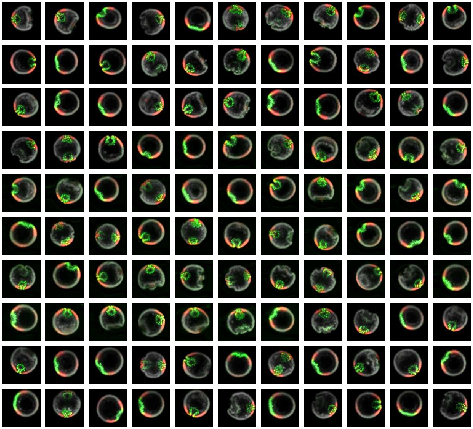
\includegraphics[width=8.4cm]{raw_data2}
\hfill
\raisebox{10.8cm}{{\figtextfont B}}
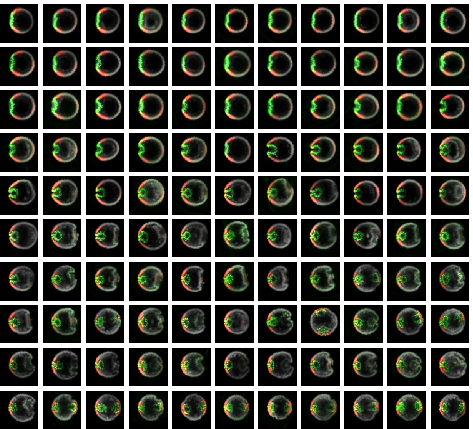
\includegraphics[width=8.4cm]{VDM_ordered} 

\vspace{0.2cm}
\centering
\raisebox{0.6cm}{{\figtextfont C}}
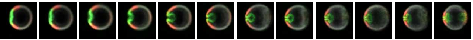
\includegraphics[width=16.8cm]{average_trajectory}

\caption{(A) Images from stages 5-7 of {\it Drosophila} embryogenesis. Each image is of a different embryo in a different rotational orientation. (B) Data from A, registered and ordered using vector diffusion maps. (C) Average trajectory of the images shown in B.}
\customlabel{fig:data2}{5}
\customlabel{subfig:raw_data2}{\ref{fig:data2}{\it A}}
\customlabel{subfig:ordered_data2}{\ref{fig:data2}{\it B}}
\customlabel{subfig:averaged_trajectory}{\ref{fig:data2}{\it C}}
\end{figure*}


\section{Conclusions}

We present algorithms for registration and temporal ordering of images.
%
The algorithms are sufficiently general that they can be applied to a wide variety of biological imaging data.

Although the examples here focus on temporally ordering the data, tasks such as classification and comparison of different mutations can also be accomplished using the same techniques. 
%

\begin{itemize}
\item What are other people doing  (maybe critically)
\item Movies  smoothness
\item Discrete symmetries like flips
\item Local information ? (features of the image) (associate with Fourier-Bessel and bispectra)
\item Mutant-wildtype stuff  IMPORTANT
\item And in general, MULTIPLE variablities is important (mutants, guys in another cycle, etc.)
 
\item size is an issue
\item  small tilts is an issue
\item   could one do three-d image processing ?  of the floating thing, without the device
\item how do we go about merging datasets ?
\end{itemize}



\bibliographystyle{pnas}
\bibliography{background_reading/references,../../references/references}

\end{article}

\end{document}

